%! Author = mddzi
%! Date = 02.06.2024

% Preamble
\documentclass[12pt,a4paper,twoside]{report}

% Packages
\usepackage{amsmath}
\usepackage[T1]{fontenc}
\usepackage[utf8]{inputenc}
\usepackage{lmodern}
\usepackage{textcomp}
\usepackage{lastpage}
\usepackage{geometry}
\usepackage{graphicx}
\usepackage{fancyhdr}
\usepackage[svgnames]{xcolor}
\usepackage[font={small,color=Grey},labelsep=period,width={0.8\textwidth}]{caption}
\usepackage{float}
\usepackage{multirow}
\usepackage{subcaption}
\usepackage{adjustbox}
\usepackage{longtable}
\usepackage{etoolbox}
\usepackage{hyperref}
\usepackage{pdfpages}
\usepackage{indentfirst}

\geometry{margin=3.5cm}

\renewcommand{\figurename}{Rysunek}
\renewcommand{\chaptername}{Rozdział}
\renewcommand{\contentsname}{Spis treści}
\renewcommand{\bibname}{Bibliografia}

\pagestyle{fancy}

\title{\textbf{Program do tworzenia schematów układów scalonych w formie gry edukacyjnej}\\[2ex]
    \large Program for creating IC diagrams in the form of an educational game\\
}
\author{Maksymilian Dziemiańczuk}
\date{}

\fancyhf{}
\fancyhead{}
\fancyhead[RO,LE]{Maksymilian Dziemiańczuk}
\fancyhead[RO,LE]{Projekt inżynierski}
\fancyfoot{}
\fancyfoot[RO,LE]{\thepage}
\fancyfoot[RE,LO]{\footnotesize Program do tworzenia schematów układów scalonych w formie gry edukacyjnej}
\fancypagestyle{plain}{
    \renewcommand{\headrulewidth}{0pt}
    \fancyhf{}
    \fancyfoot[RO,LE]{\thepage}
    \fancyfoot[RE,LO]{\footnotesize Program do tworzenia schematów układów scalonych w formie gry edukacyjnej}
}

% Document
\begin{document}

%\maketitle
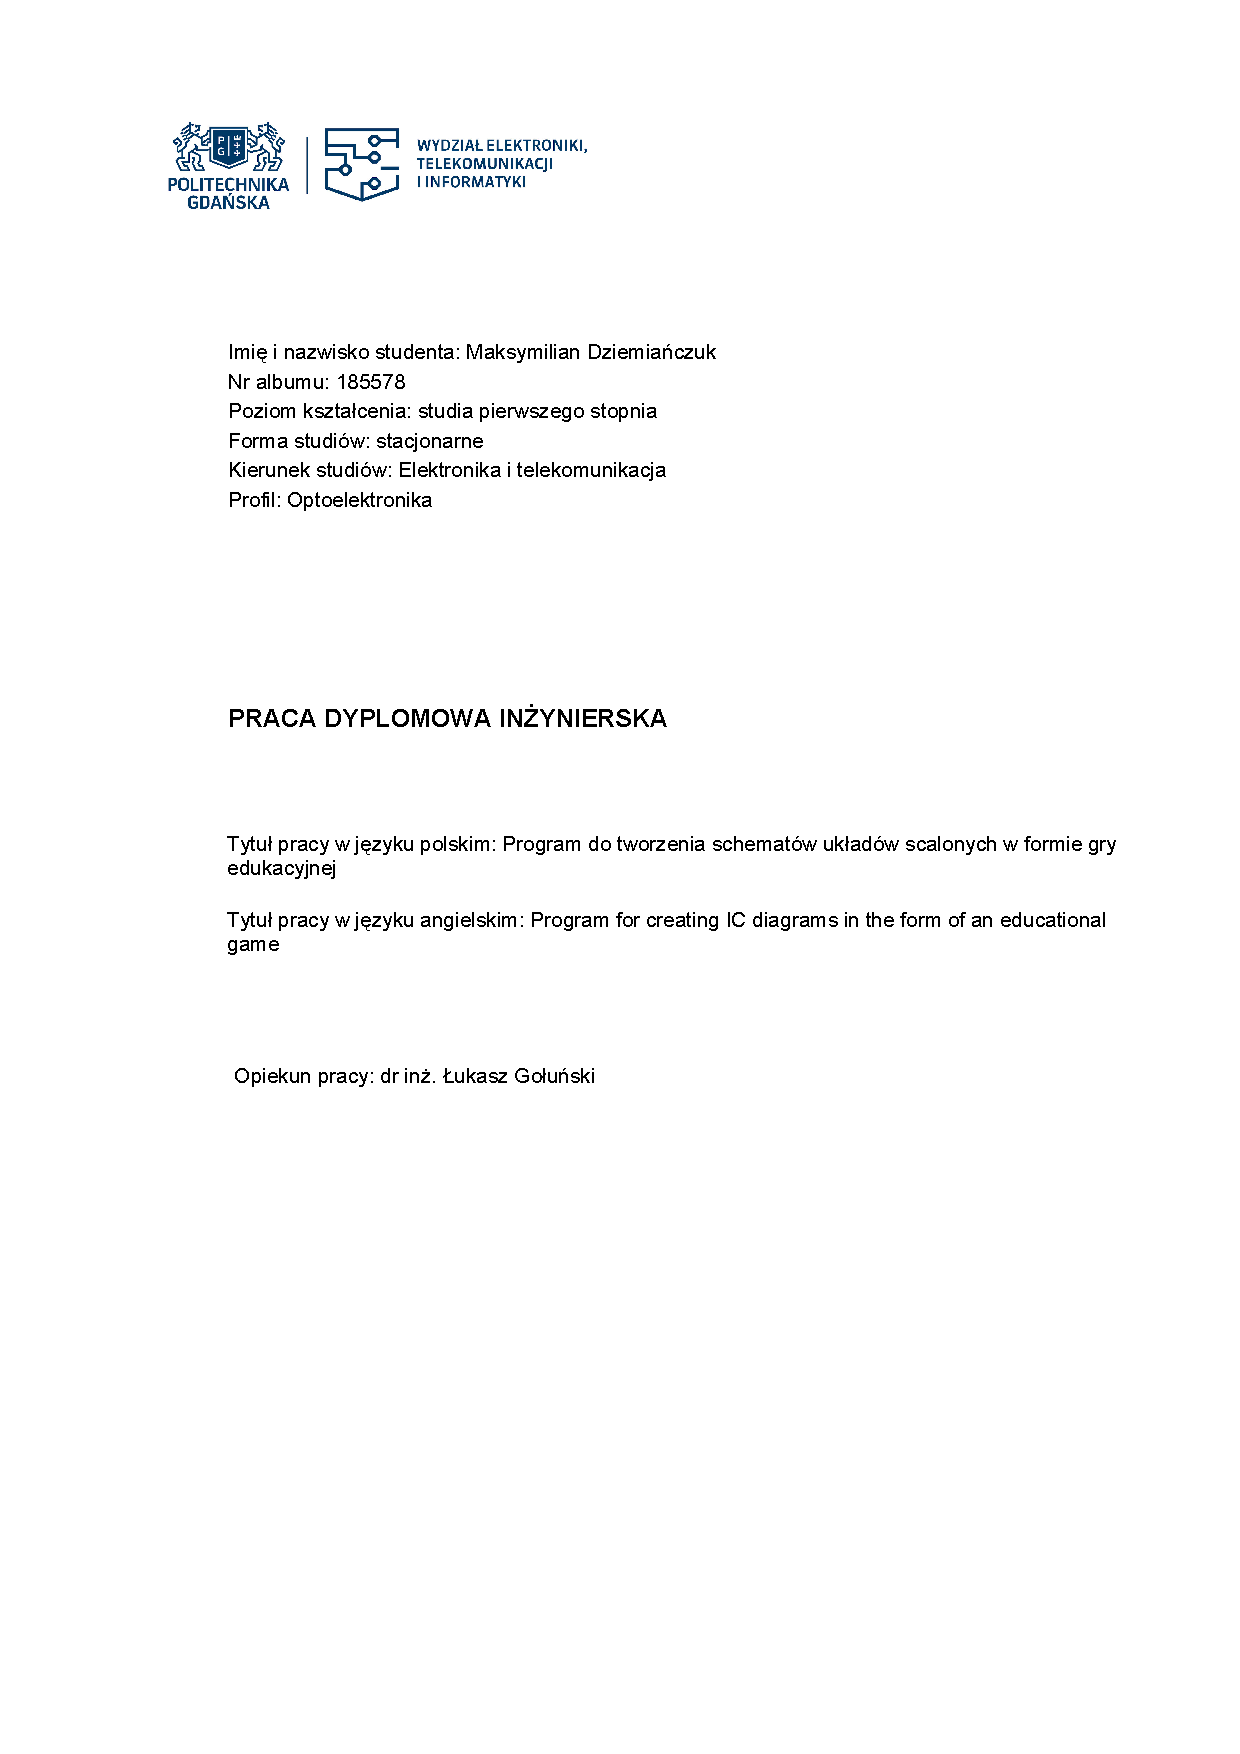
\includepdf[pages={1}]{StronaTytulowa_185578.pdf}

%pusta strona
\newpage \thispagestyle{empty} \ \newpage

\section*{Streszczenie}
\thispagestyle{plain}

Lorem ipsum dolor sit amet, consectetur adipiscing elit

\tableofcontents

\chapter{Wstęp i cel pracy}
Programy do tworzenia schematów są jednym z kluczowych elementów
procesu wielkoskalowej integracji układów scalonych (ang. VLSI — Very Large Scale Integration)\cite{VLSI}.
Polega to na projektowaniu podukładów o określonych funkcjach,
które następnie są łączone w jeden, w pełni działający układ scalony.
W ten sposób upraszczany jest proces projektowania oraz produkcji układów scalonych,
gdyż pracę można podzielić na mniejsze części,
a dodatkowo cześć podukładów może być używana w wielu różnych projektach.
Przykładem takiego programu jest open-source'owy, MAGIC VLSI stworzony przez Johna Ousterhouta w 1980 roku\cite{MAGIC},
napisany w języku C na platformę Linux\cite{MAGIC_wiki}.
Charakteryzuje go prosta szata graficzna oraz szeroki zakres działania,
natomiast jego obsługa bywa często nieintuicyjna oraz nieprzyjazna dla początkujących użytkowników
co stało się inspiracją dla tego projektu.\\
\indent Ze względu na wysoki próg wejścia programów takich jak MAGIC, celem tego projektu było stworzenie
programu edukacyjnego w formie gry, który pomoże w nauce tworzenia schematów układów scalonych.
%
Jedne z głównych założeń to prostota obsługi, intuicyjność oraz wysoka ergonomia,
na które mają wpływ przede wszystkim dobrze zaprojektowany interfejs graficzny użytkownika
oraz wbudowane narzędzia ułatwiające edycję schematu.
Na tych założeniach opiera się cała część projektu związana z interfejsem użytkownika.\\
%
\indent Kolejnym istotnym elementem tej pracy było przygotowanie angażującej i skalowalnej pętli rozgrywki,
która pozwoli na stopniowe wprowadzanie użytkownika w projektowanie schematów układów scalonych,
wraz z implementacją systemów sprawdzania poprawności wykonanych zadań, wskazywania błędów i ewentualnych podpowiedzi.
Dzięki realizacji założeń program pomoże w nauce podstaw bez odrzucania użytkownika
przez zbyt skomplikowaną obsługę.
%Aby ujednolicić schematy oraz zadania do wykonania dla użytkowników,
%projektowanie będzie odbywać się w tylko jednej technologii\ \textendash \ CMOS AMIS ami-C5.
%Powodem wyboru tej technologii jest wcześniejsze doświadczenie w projektowaniu schematów układów scalonych
%w tej technologii.


%\LaTeX{} \cite{VLSI} is a set of macros built atop \TeX{} \cite{texbook}.

    \bibliography{main}
    \bibliographystyle{plain}

\end{document}
